\documentclass[12pt,a4paper]{article}

\usepackage[UTF8]{ctex}
\usepackage[scale=0.8]{geometry}
\usepackage{latexsym,amsmath,amsfonts,amssymb,mathrsfs,bm}
\usepackage{abstract,appendix,titlesec,titletoc}
\usepackage{diagbox,booktabs,longtable,tabularx}
\usepackage[amsmath,thmmarks,hyperref]{ntheorem}
\usepackage{fancyhdr,indentfirst}
\usepackage[colorlinks=ture]{hyperref}
\usepackage{makeidx,cleveref}
\usepackage[sort&compress, numbers]{natbib}
\usepackage{graphicx,epsfig,subfig}
\usepackage{algorithm,algorithmicx,algpseudocode}
\usepackage{xcolor}

\linespread{1.3}
\setlength{\parskip}{0.5\baselineskip}

\theoremstyle{plain}
\newtheorem{definition}{定义}
\newtheorem{example}{例}
\newtheorem{theorem}{定理}
\newtheorem{lemma}{引理}
\newtheorem{corollary}{推论}
\newtheorem{remark}{注}
\newtheorem{proposition}{性质}

\newcommand{\Rnum}{\mathbb{R}}
\newcommand{\Cnum}{\mathbb{C}}
\newcommand{\Znum}{\mathbb{Z}}
\newcommand{\Nnum}{\mathbb{N}}
\newcommand{\Prob}{\mathbb{P}}
\newcommand{\bx}{\mathbf{x}}
\newcommand{\by}{\mathbf{y}}
\newcommand{\bn}{\mathbf{n}}

\title{用PPR技术重构梯度}
\date{\today}

\begin{document}

\maketitle

我们构造了任意网格上的边中点有限体积格式,数值解的未知量定义在边中点,可以达到二阶精度。现在希望通过边中点信息重构导数信息。

\subsection*{PPR技术}

对于原始网格中的某个网格点$A$(图中红色),可以找出它附近单元中的所有边。这些边的中点(图中绿色)记为$\mathcal{E}$。不考虑边界和界面上的网格点。如图,对于扭曲的三角形和四边形网格,每个节点周围都是用12个边中点拟合$P_2$多项式,自由度一定够用。

对于某个网格边中点$A$(图中红色),我们可以用同样的方法找出它附近单元对应的边中点(包括自身)。对于三角形网格,边中点的个数不够,需要继续扩张,得到13个边中点。而对于四边形网格,可以得到7个边中点。

\begin{figure}[H]
\centering
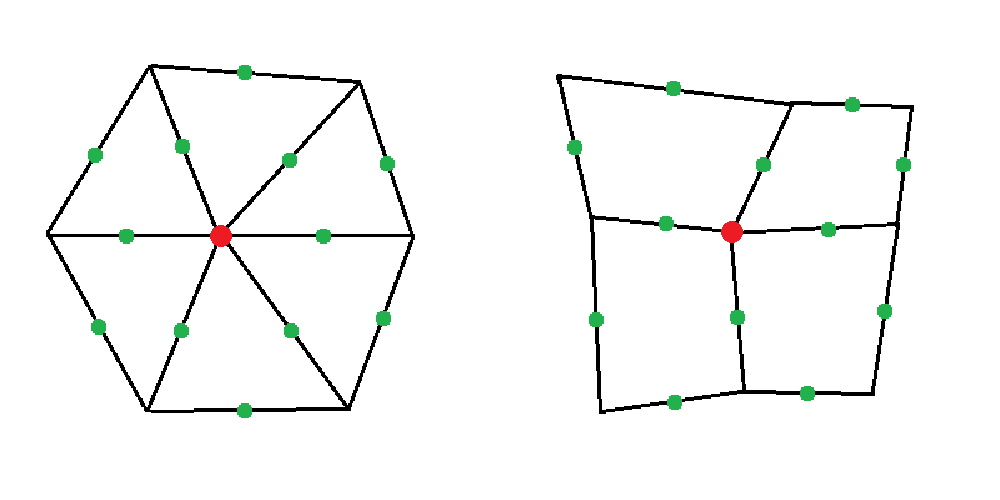
\includegraphics[width=0.49\linewidth]{stencil1}
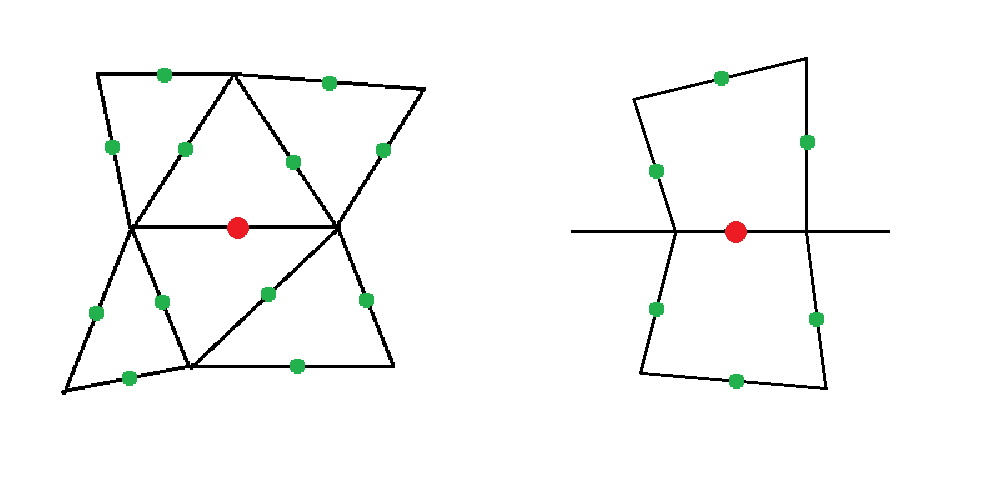
\includegraphics[width=0.49\linewidth]{stencil2}
\caption{PPR模板}
\end{figure}

对于扩散系数连续的情况,我们用二次多项式对所有边中点做最小二乘拟合,相当于求解优化问题
\begin{align*}
\min_{p \in P_2} \sum_{E \in \mathcal{E}} |p(\bm{x}_E) - u_E|^2
\end{align*}
得到多项式$p(x)$,此时它的梯度$(\mathcal{G} u) (A) = \nabla p(A)$就是$A$处关于梯度的重构。

重构得到的梯度$(\mathcal{G} u) (A)$和真实的梯度$\nabla u(A)$之间应该具有二阶精度。

然后,我们可以计算出$A$处的流量为$\Lambda \, (\mathcal{G} u) (A)$。

这样做可能会破坏守恒性,重构出来的流量不满足在原始网格上守恒。

对于节点位于界面上的情况,我们觉得可以在界面的两边分别拟合两个二次多项式,同时利用流连续条件把两个多项式拼起来。这个想法还没有实现。

\subsection*{数值结果}

\begin{figure}[h]
\centering
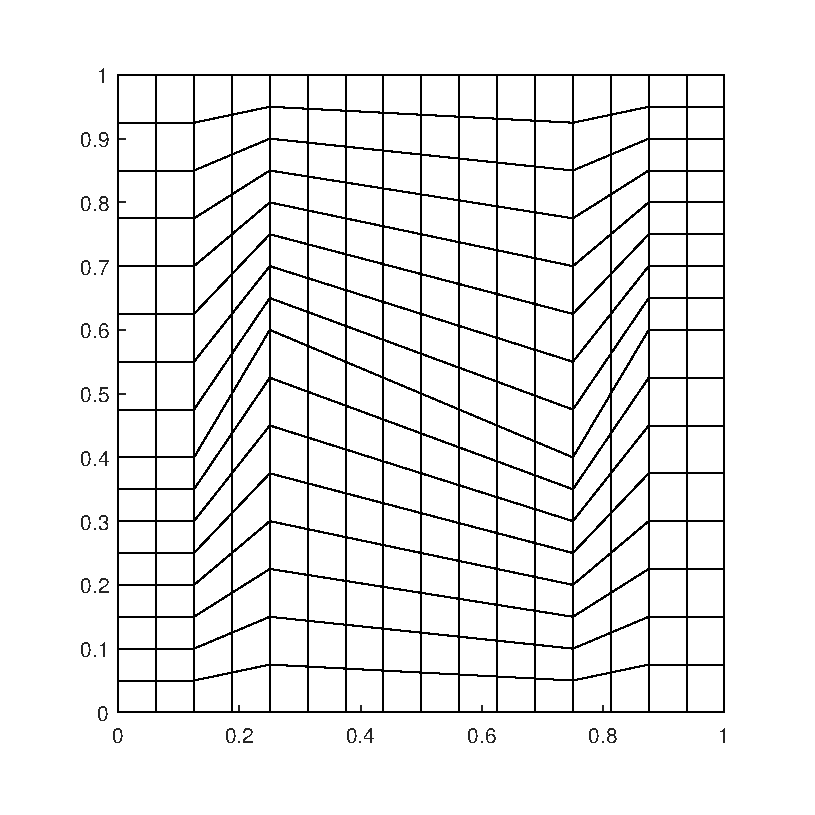
\includegraphics[width=0.3\linewidth]{m4}
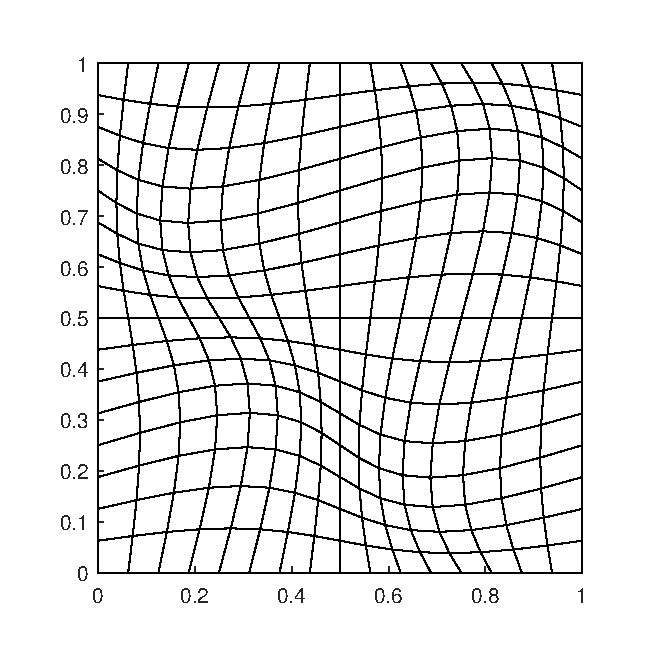
\includegraphics[width=0.3\linewidth]{m3}
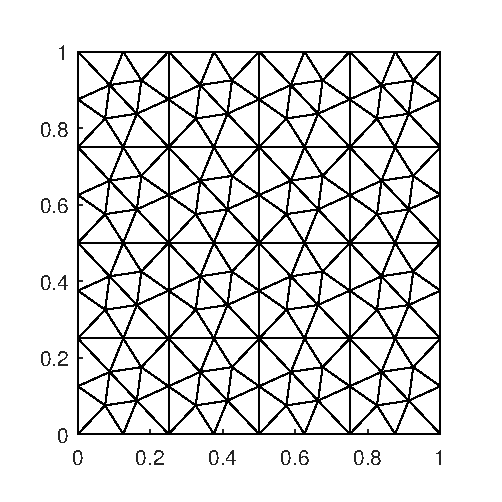
\includegraphics[width=0.3\linewidth]{m5}
\caption{实验中用到的网格}
\end{figure}

我们找了一个很简单的例子。精确解和系数选为
\begin{align*}
u = 16 \, x \, y \, (1-x) \, (1-y) \qquad
a = \left[
\begin{matrix}
1.5 & 0.5 \\
0.5 & 1.5 \\
\end{matrix}
\right]
\end{align*}

表里面的符号$\|\nabla u - \mathcal{G} u\|_\infty$表示把精确解当作输入,用PPR方法重构梯度的误差。$\|\nabla u - \mathcal{G} u_h\|_\infty$表示用PPR方法重构数值解的梯度误差。

\newpage
\subsection*{重构节点上的梯度}

首先我们尝试在均匀的正方形网格上求解问题,结果在表1中。在网格没有任何扭曲的时候,各种方法都能达到二阶精度。

\begin{table}[h]
\centering
\scriptsize
\begin{tabular}{r|cc|cc|cc|cc|cc}
\hline
& \multicolumn{2}{c|}{exact} & \multicolumn{4}{c}{ECS-I} & \multicolumn{4}{|c}{ECS-II} \\
\hline
DoF & $\|\nabla u - \mathcal{G} u\|_\infty$ & order & $\|u - u_h\|_\infty$ & order & $\|\nabla u - \mathcal{G} u_h\|_\infty$ & order & $\|u - u_h\|_\infty$ & order & $\|\nabla u - \mathcal{G} u_h\|_\infty$ & order \\
\hline
40 & 1.82e-01 & NaN & 3.24e-02 & NaN & 1.37e-01 & NaN & 2.92e-02 & NaN & 1.44e-01 & NaN \\
144 & 6.82e-02 & 1.53 & 8.31e-03 & 2.12 & 5.77e-02 & 1.34 & 7.54e-03 & 2.11 & 5.43e-02 & 1.52 \\
544 & 1.99e-02 & 1.85 & 2.09e-03 & 2.08 & 1.82e-02 & 1.74 & 1.92e-03 & 2.06 & 1.59e-02 & 1.85 \\
2112 & 5.33e-03 & 1.94 & 5.23e-04 & 2.04 & 5.08e-03 & 1.88 & 4.84e-04 & 2.03 & 4.27e-03 & 1.94 \\
8320 & 1.38e-03 & 1.97 & 1.31e-04 & 2.02 & 1.34e-03 & 1.94 & 1.22e-04 & 2.02 & 1.10e-03 & 1.97 \\
33024 & 3.50e-04 & 1.99 & 3.27e-05 & 2.01 & 3.45e-04 & 1.97 & 3.04e-05 & 2.01 & 2.80e-04 & 1.99 \\
\hline
\end{tabular}
\caption{正方形网格 重构节点处的梯度}
\end{table}

然后我们尝试把网格轻微扭曲一下,如图2的第一张图所示。网格变形的程度很小,收敛阶在表2中展示。
从表中可以看出,用精确解重构的梯度还是二阶的,一定程度上可以说明代码没有问题。但是在这样的网格上,PPR方法重构的数值解梯度就是一阶的。这个结果和我们的预期不符。

\begin{table}[h]
\centering
\scriptsize
\begin{tabular}{r|cc|cc|cc|cc|cc}
\hline
& \multicolumn{2}{c|}{exact} & \multicolumn{4}{c}{ECS-I} & \multicolumn{4}{|c}{ECS-II} \\
\hline
DoF & $\|\nabla u - \mathcal{G} u\|_\infty$ & order & $\|u - u_h\|_\infty$ & order & $\|\nabla u - \mathcal{G} u_h\|_\infty$ & order & $\|u - u_h\|_\infty$ & order & $\|\nabla u - \mathcal{G} u_h\|_\infty$ & order \\
\hline
40 & 1.86e-01 & NaN & 3.70e-02 & NaN & 1.52e-01 & NaN & 5.38e-02 & NaN & 1.65e-01 & NaN \\
144 & 8.93e-02 & 1.15 & 1.58e-02 & 1.33 & 8.79e-02 & 0.85 & 1.57e-02 & 1.92 & 8.45e-02 & 1.04 \\
544 & 4.13e-02 & 1.16 & 4.21e-03 & 1.99 & 4.94e-02 & 0.87 & 5.43e-03 & 1.60 & 4.54e-02 & 0.94 \\
2112 & 1.27e-02 & 1.74 & 1.08e-03 & 2.00 & 2.15e-02 & 1.22 & 1.55e-03 & 1.85 & 1.37e-02 & 1.76 \\
8320 & 3.55e-03 & 1.86 & 3.07e-04 & 1.84 & 1.20e-02 & 0.86 & 4.13e-04 & 1.93 & 6.49e-03 & 1.09 \\
33024 & 9.39e-04 & 1.93 & 8.17e-05 & 1.92 & 6.32e-03 & 0.93 & 1.06e-04 & 1.97 & 3.31e-03 & 0.97 \\
\hline
\end{tabular}
\caption{Kershaw四边形网格 重构节点处的梯度}
\end{table}

但是在另一种四边形网格上,如图2第二张图所示。这样扭曲得到的网格比较平滑,收敛阶在这上面就又变成二阶的了。这样的现象很神奇,我们也不知道怎么解释。

\begin{table}[h]
\centering
\scriptsize
\begin{tabular}{r|cc|cc|cc|cc|cc}
\hline
& \multicolumn{2}{c|}{exact} & \multicolumn{4}{c}{ECS-I} & \multicolumn{4}{|c}{ECS-II} \\
\hline
DoF & $\|\nabla u - \mathcal{G} u\|_\infty$ & order & $\|u - u_h\|_\infty$ & order & $\|\nabla u - \mathcal{G} u_h\|_\infty$ & order & $\|u - u_h\|_\infty$ & order & $\|\nabla u - \mathcal{G} u_h\|_\infty$ & order \\
\hline
40 & 2.29e-01 & NaN & 4.91e-02 & NaN & 1.77e-01 & NaN & 4.22e-02 & NaN & 1.81e-01 & NaN \\
144 & 1.15e-01 & 1.07 & 1.49e-02 & 1.86 & 1.09e-01 & 0.75 & 1.44e-02 & 1.68 & 1.05e-01 & 0.85 \\
544 & 3.98e-02 & 1.59 & 3.82e-03 & 2.05 & 3.74e-02 & 1.61 & 4.18e-03 & 1.86 & 3.64e-02 & 1.59 \\
2112 & 1.15e-02 & 1.83 & 9.76e-04 & 2.01 & 1.12e-02 & 1.78 & 1.10e-03 & 1.97 & 1.04e-02 & 1.85 \\
8320 & 3.02e-03 & 1.95 & 2.45e-04 & 2.01 & 3.10e-03 & 1.87 & 2.80e-04 & 2.00 & 2.79e-03 & 1.91 \\
33024 & 7.68e-04 & 1.98 & 6.14e-05 & 2.01 & 8.20e-04 & 1.93 & 7.04e-05 & 2.00 & 7.26e-04 & 1.96 \\
\hline
\end{tabular}
\caption{Sin四边形网格 重构节点处的梯度}
\end{table}

最后我们尝试了三角形网格,两种边格式在三角形网格上是等价的。计算的结果在表4中。三角形网格上表现出来的结果和扭曲四边形相同。都没有达到二阶。

\begin{table}[h]
\centering
\scriptsize
\begin{tabular}{r|cc|cc|cc}
\hline
& \multicolumn{2}{c|}{exact} & \multicolumn{4}{c}{ECS-I} \\
\hline
DoF & $\|\nabla u - \mathcal{G} u\|_\infty$ & order & $\|u - u_h\|_\infty$ & order & $\|\nabla u - \mathcal{G} u_h\|_\infty$ & order \\
\hline
92 & 8.45e-02 & * & 5.43e-02 & * & 6.19e-02 & * \\
352 & 2.70e-02 & 1.70 & 1.77e-02 & 1.67 & 2.88e-02 & 1.14 \\
1376 & 8.55e-03 & 1.69 & 4.96e-03 & 1.86 & 1.47e-02 & 0.99 \\
5440 & 2.49e-03 & 1.79 & 1.31e-03 & 1.94 & 7.42e-03 & 1.00 \\
21632 & 6.68e-04 & 1.91 & 3.37e-04 & 1.97 & 3.72e-03 & 1.00 \\
86272 & 1.73e-04 & 1.96 & 8.54e-05 & 1.98 & 1.86e-03 & 1.00 \\
\hline
\end{tabular}
\caption{三角形网格 重构节点处的梯度}
\end{table}

\newpage
\subsection*{重构边中点的梯度}

随后我们认为这样的现象可能是重构梯度的位置和数值解定义的位置不匹配造成的。于是我们尝试重构各边中点处的梯度。如表4所示。在正方形网格上,仍然是二阶的。

\begin{table}[h]
\centering
\scriptsize
\begin{tabular}{r|cc|cc|cc|cc|cc}
\hline
& \multicolumn{2}{c|}{exact} & \multicolumn{4}{c}{ECS-I} & \multicolumn{4}{|c}{ECS-II} \\
\hline
DoF & $\|\nabla u - \mathcal{G} u\|_\infty$ & order & $\|u - u_h\|_\infty$ & order & $\|\nabla u - \mathcal{G} u_h\|_\infty$ & order & $\|u - u_h\|_\infty$ & order & $\|\nabla u - \mathcal{G} u_h\|_\infty$ & order \\
\hline
40 & 8.11e-01 & NaN & 3.24e-02 & NaN & 7.06e-01 & NaN & 2.92e-02 & NaN & 6.77e-01 & NaN \\
144 & 2.37e-01 & 1.92 & 8.31e-03 & 2.12 & 2.18e-01 & 1.84 & 7.54e-03 & 2.11 & 1.97e-01 & 1.93 \\
544 & 6.34e-02 & 1.98 & 2.09e-03 & 2.08 & 6.05e-02 & 1.93 & 1.92e-03 & 2.06 & 5.27e-02 & 1.99 \\
2112 & 1.64e-02 & 2.00 & 5.23e-04 & 2.04 & 1.60e-02 & 1.96 & 4.84e-04 & 2.03 & 1.36e-02 & 2.00 \\
8320 & 4.16e-03 & 2.00 & 1.31e-04 & 2.02 & 4.11e-03 & 1.98 & 1.22e-04 & 2.02 & 3.44e-03 & 2.00 \\
33024 & 1.05e-03 & 2.00 & 3.27e-05 & 2.01 & 1.04e-03 & 1.99 & 3.04e-05 & 2.01 & 2.62e-03 & 0.39 \\
\hline
\end{tabular}
\caption{正方形网格 重构边中点处的梯度}
\end{table}

然后我们尝试在扭曲的Kershaw网格上,收敛阶在表6中展示。不知道为什么,用精确解重构的梯度变成了一阶的,而用数值解重构的梯度直接没有阶了。我们目前还没在代码里找到错误。

\begin{table}[h]
\centering
\scriptsize
\begin{tabular}{r|cc|cc|cc|cc|cc}
\hline
& \multicolumn{2}{c|}{exact} & \multicolumn{4}{c}{ECS-I} & \multicolumn{4}{|c}{ECS-II} \\
\hline
DoF & $\|\nabla u - \mathcal{G} u\|_\infty$ & order & $\|u - u_h\|_\infty$ & order & $\|\nabla u - \mathcal{G} u_h\|_\infty$ & order & $\|u - u_h\|_\infty$ & order & $\|\nabla u - \mathcal{G} u_h\|_\infty$ & order \\
\hline
40 & 2.29e-01 & NaN & 3.70e-02 & NaN & 1.90e-01 & NaN & 5.38e-02 & NaN & 2.31e-01 & NaN \\
144 & 4.58e-01 & -1.09 & 1.58e-02 & 1.33 & 1.79e+00 & -3.50 & 1.57e-02 & 1.92 & 3.48e-01 & -0.64 \\
544 & 2.84e-01 & 0.72 & 4.21e-03 & 1.99 & 1.90e+00 & -0.09 & 5.43e-03 & 1.60 & 7.92e-01 & -1.24 \\
2112 & 1.58e-01 & 0.86 & 1.08e-03 & 2.00 & 1.22e+00 & 0.65 & 1.55e-03 & 1.85 & 7.77e-01 & 0.03 \\
8320 & 8.35e-02 & 0.93 & 3.07e-04 & 1.84 & 1.71e+00 & -0.49 & 4.13e-04 & 1.93 & 7.99e-01 & -0.04 \\
33024 & 4.29e-02 & 0.97 & 8.17e-05 & 1.92 & 2.75e+00 & -0.69 & 1.06e-04 & 1.97 & 6.21e-01 & 0.37 \\
\hline
\end{tabular}
\caption{Kershaw四边形网格 重构边中点处的梯度}
\end{table}

在sin四边形网格上,就可以达到二阶。同样是扭曲的四边形网格,不同的扭曲方式居然会带来不同的结果。我们觉得这很神奇。

\begin{table}[h]
\centering
\scriptsize
\begin{tabular}{r|cc|cc|cc|cc|cc}
\hline
& \multicolumn{2}{c|}{exact} & \multicolumn{4}{c}{ECS-I} & \multicolumn{4}{|c}{ECS-II} \\
\hline
DoF & $\|\nabla u - \mathcal{G} u\|_\infty$ & order & $\|u - u_h\|_\infty$ & order & $\|\nabla u - \mathcal{G} u_h\|_\infty$ & order & $\|u - u_h\|_\infty$ & order & $\|\nabla u - \mathcal{G} u_h\|_\infty$ & order \\
\hline
40 & 2.36e-01 & NaN & 4.91e-02 & NaN & 1.45e-01 & NaN & 4.22e-02 & NaN & 1.41e-01 & NaN \\
144 & 8.21e-02 & 1.65 & 1.49e-02 & 1.86 & 9.08e-02 & 0.73 & 1.44e-02 & 1.68 & 8.54e-02 & 0.78 \\
544 & 2.78e-02 & 1.63 & 3.82e-03 & 2.05 & 2.85e-02 & 1.75 & 4.18e-03 & 1.86 & 2.83e-02 & 1.66 \\
2112 & 7.88e-03 & 1.86 & 9.76e-04 & 2.01 & 8.36e-03 & 1.81 & 1.10e-03 & 1.97 & 7.65e-03 & 1.93 \\
8320 & 2.07e-03 & 1.95 & 2.45e-04 & 2.01 & 2.32e-03 & 1.87 & 2.80e-04 & 2.00 & 1.99e-03 & 1.96 \\
33024 & 5.27e-04 & 1.98 & 6.14e-05 & 2.01 & 6.18e-04 & 1.92 & 7.04e-05 & 2.00 & 5.08e-04 & 1.98 \\
\hline
\end{tabular}
\caption{Sin四边形网格 重构边中点处的梯度}
\end{table}

最后我们尝试了三角形网格,两种边格式在三角形网格上是等价的。计算的结果在表8中。三角形网格上表现出来的结果和之前相同。重构的数值解梯度也没有达到二阶。

\begin{table}[h]
\centering
\scriptsize
\begin{tabular}{r|cc|cc|cc}
\hline
& \multicolumn{2}{c|}{exact} & \multicolumn{4}{c}{ECS-I} \\
\hline
DoF & $\|\nabla u - \mathcal{G} u\|_\infty$ & order & $\|u - u_h\|_\infty$ & order & $\|\nabla u - \mathcal{G} u_h\|_\infty$ & order \\
\hline
92 & 2.17e-01 & NaN & 5.43e-02 & NaN & 4.04e-01 & NaN \\
352 & 6.23e-02 & 1.86 & 1.77e-02 & 1.67 & 1.85e-01 & 1.16 \\
1376 & 1.66e-02 & 1.94 & 4.96e-03 & 1.86 & 8.64e-02 & 1.12 \\
5440 & 4.27e-03 & 1.97 & 1.31e-03 & 1.94 & 4.13e-02 & 1.07 \\
21632 & 1.08e-03 & 1.99 & 3.37e-04 & 1.97 & 2.01e-02 & 1.04 \\
86272 & 2.73e-04 & 1.99 & 8.54e-05 & 1.98 & 9.94e-03 & 1.02 \\
\hline
\end{tabular}
\caption{三角形网格 重构边中点处的梯度}
\end{table}

\newpage
\subsection*{通过节点重构边上的梯度}

在原先的文献中,边中点的梯度不是直接计算得到的,而是通过先重构节点处的梯度,然后在边中点处插值得到的。我们也尝试了这种方法。

在正方形网格上,一切都很顺利。

\begin{table}[h]
\centering
\scriptsize
\begin{tabular}{r|cc|cc|cc|cc|cc}
\hline
& \multicolumn{2}{c|}{exact} & \multicolumn{4}{c}{ECS-I} & \multicolumn{4}{|c}{ECS-II} \\
\hline
DoF & $\|\nabla u - \mathcal{G} u\|_\infty$ & order & $\|u - u_h\|_\infty$ & order & $\|\nabla u - \mathcal{G} u_h\|_\infty$ & order & $\|u - u_h\|_\infty$ & order & $\|\nabla u - \mathcal{G} u_h\|_\infty$ & order \\
\hline
40 & 3.07e-01 & NaN & 3.24e-02 & NaN & 2.53e-01 & NaN & 2.92e-02 & NaN & 2.68e-01 & NaN \\
144 & 1.15e-01 & 1.53 & 8.31e-03 & 2.12 & 1.01e-01 & 1.44 & 7.54e-03 & 2.11 & 1.01e-01 & 1.52 \\
544 & 3.36e-02 & 1.85 & 2.09e-03 & 2.08 & 3.11e-02 & 1.77 & 1.92e-03 & 2.06 & 2.96e-02 & 1.85 \\
2112 & 8.99e-03 & 1.94 & 5.23e-04 & 2.04 & 8.62e-03 & 1.89 & 4.84e-04 & 2.03 & 7.93e-03 & 1.94 \\
8320 & 2.32e-03 & 1.97 & 1.31e-04 & 2.02 & 2.27e-03 & 1.95 & 1.22e-04 & 2.02 & 2.05e-03 & 1.97 \\
33024 & 5.90e-04 & 1.99 & 3.27e-05 & 2.01 & 5.83e-04 & 1.97 & 3.04e-05 & 2.01 & 5.21e-04 & 1.99 \\
\hline
\end{tabular}
\caption{正方形网格 通过节点重构边上的梯度}
\end{table}

然后我们尝试在扭曲的Kershaw网格上,用数值解重构的梯度还是一阶的,和直接重构节点处的梯度相同。

\begin{table}[h]
\centering
\scriptsize
\begin{tabular}{r|cc|cc|cc|cc|cc}
\hline
& \multicolumn{2}{c|}{exact} & \multicolumn{4}{c}{ECS-I} & \multicolumn{4}{|c}{ECS-II} \\
\hline
DoF & $\|\nabla u - \mathcal{G} u\|_\infty$ & order & $\|u - u_h\|_\infty$ & order & $\|\nabla u - \mathcal{G} u_h\|_\infty$ & order & $\|u - u_h\|_\infty$ & order & $\|\nabla u - \mathcal{G} u_h\|_\infty$ & order \\
\hline
40 & 3.61e-01 & NaN & 3.70e-02 & NaN & 3.60e-01 & NaN & 5.38e-02 & NaN & 3.60e-01 & NaN \\
144 & 1.58e-01 & 1.29 & 1.58e-02 & 1.33 & 1.56e-01 & 1.31 & 1.57e-02 & 1.92 & 1.52e-01 & 1.34 \\
544 & 5.98e-02 & 1.46 & 4.21e-03 & 1.99 & 6.25e-02 & 1.37 & 5.43e-03 & 1.60 & 6.23e-02 & 1.34 \\
2112 & 2.02e-02 & 1.60 & 1.08e-03 & 2.00 & 2.12e-02 & 1.59 & 1.55e-03 & 1.85 & 2.08e-02 & 1.62 \\
8320 & 5.72e-03 & 1.84 & 3.07e-04 & 1.84 & 1.15e-02 & 0.89 & 4.13e-04 & 1.93 & 6.78e-03 & 1.63 \\
33024 & 1.53e-03 & 1.92 & 8.17e-05 & 1.92 & 6.22e-03 & 0.89 & 1.06e-04 & 1.97 & 3.47e-03 & 0.97 \\
\hline
\end{tabular}
\caption{Kershaw四边形网格 通过节点重构边上的梯度}
\end{table}

在sin四边形网格上,就可以达到二阶。

\begin{table}[h]
\centering
\scriptsize
\begin{tabular}{r|cc|cc|cc|cc|cc}
\hline
& \multicolumn{2}{c|}{exact} & \multicolumn{4}{c}{ECS-I} & \multicolumn{4}{|c}{ECS-II} \\
\hline
DoF & $\|\nabla u - \mathcal{G} u\|_\infty$ & order & $\|u - u_h\|_\infty$ & order & $\|\nabla u - \mathcal{G} u_h\|_\infty$ & order & $\|u - u_h\|_\infty$ & order & $\|\nabla u - \mathcal{G} u_h\|_\infty$ & order \\
\hline
40 & 4.31e-01 & NaN & 4.91e-02 & NaN & 3.67e-01 & NaN & 4.22e-02 & NaN & 3.79e-01 & NaN \\
144 & 1.72e-01 & 1.44 & 1.49e-02 & 1.86 & 1.59e-01 & 1.31 & 1.44e-02 & 1.68 & 1.57e-01 & 1.38 \\
544 & 5.97e-02 & 1.59 & 3.82e-03 & 2.05 & 5.74e-02 & 1.53 & 4.18e-03 & 1.86 & 5.62e-02 & 1.54 \\
2112 & 1.85e-02 & 1.73 & 9.76e-04 & 2.01 & 1.77e-02 & 1.73 & 1.10e-03 & 1.97 & 1.72e-02 & 1.75 \\
8320 & 4.99e-03 & 1.91 & 2.45e-04 & 2.01 & 4.98e-03 & 1.85 & 2.80e-04 & 2.00 & 4.72e-03 & 1.88 \\
33024 & 1.28e-03 & 1.97 & 6.14e-05 & 2.01 & 1.32e-03 & 1.93 & 7.04e-05 & 2.00 & 1.23e-03 & 1.95 \\
\hline
\end{tabular}
\caption{Sin四边形网格 通过节点重构边上的梯度}
\end{table}

在三角形网格上看起来也没有二阶。这里的误差比直接重构节点梯度更小,但是定性的结论上都是吻合的。

\begin{table}[hb]
\centering
\scriptsize
\begin{tabular}{r|cc|cc|cc}
\hline
& \multicolumn{2}{c|}{exact} & \multicolumn{4}{c}{ECS-I} \\
\hline
DoF & $\|\nabla u - \mathcal{G} u\|_\infty$ & order & $\|u - u_h\|_\infty$ & order & $\|\nabla u - \mathcal{G} u_h\|_\infty$ & order \\
\hline
92 & 3.45e-01 & NaN & 5.43e-02 & NaN & 3.33e-01 & NaN \\
352 & 9.73e-02 & 1.89 & 1.77e-02 & 1.67 & 9.76e-02 & 1.83 \\
1376 & 2.60e-02 & 1.94 & 4.96e-03 & 1.86 & 2.79e-02 & 1.84 \\
5440 & 7.34e-03 & 1.84 & 1.31e-03 & 1.94 & 8.28e-03 & 1.77 \\
21632 & 1.94e-03 & 1.93 & 3.37e-04 & 1.97 & 3.60e-03 & 1.21 \\
86272 & 4.99e-04 & 1.97 & 8.54e-05 & 1.98 & 1.66e-03 & 1.12 \\
\hline
\end{tabular}
\caption{三角形网格 通过节点重构边上的梯度}
\end{table}

\newpage
我们仔细研究了PPR方法的相关文献,二阶收敛性的证明依赖于数值解的超收敛性质。我们猜测,有限体积方法得到的数值解可能不具有和有限元类似的超收敛性质,或者超收敛性质对网格的依赖比较强,过于扭曲的网格无法满足超收敛的要求。更深入的原因可能需要进一步研究。


%\bibliographystyle{plain}
%\bibliography{FVM}

\end{document}